\section{Results}

The system was successfully implemented and validated across all major functional blocks:
hardware-driven neural signal acquisition across a configurable selection of 1--16 channels,
charge-balanced biphasic electrical stimulation, and bidirectional BLE command and data
transfer. Key quantitative results are summarised here; detailed measurements and figures
are presented in the subsections that follow.

BLE throughput with real SPI data from the Intan RHS2116 reached \TODO{X}\,kbps in the
default 16-channel configuration at 2\,kHz per channel, confirming that the hardware-driven
pipeline sustains the required data rate under continuous operation
(Section~\ref{sec:results_ble}). The stimulation pipeline was validated by oscilloscope
measurement of the biphasic waveform at the Intan RHS2116 output, confirming correct pulse
shape, timing, and charge balance across a range of configured parameters
(Section~\ref{sec:results_stim}). Multi-channel neural signal recording was confirmed by
live acquisition from the RHS2116, with all configured channels rendered in real time in
the GUI (Section~\ref{sec:results_recording}).

Power consumption of the nRF52832 peripheral module was measured at 18.6\,mW under
continuous 16-channel recording at 2\,kHz per channel at the measured supply voltage
of 3.020\,V (equivalent to 20.4\,mW at a nominal 3.3\,V). This compares favourably
with the 29.4\,mW at 3.3\,V reported by the prior single-channel
implementation~\cite{prior_impl}: at a common reference voltage of 3.3\,V, the present
work achieves a 31\,\% reduction in module power while simultaneously increasing the
channel count 16-fold. Two architectural improvements account for this: the PPI/DMA
acquisition pipeline allows the CPU to remain in low-power sleep between BLE events
rather than spinning in a polling loop, and removal of the UART peripheral eliminates
a further source of continuous power draw. Combined power consumption of the nRF52832
and Intan RHS2116 was measured at 61.3\,mW at 3.6\,V in the same 16-channel,
2\,kHz per channel configuration. Power measurements are presented in
Section~\ref{sec:results_power}.

\subsection{Neural Signal Recording}
\label{sec:results_recording}

\TODO{}

\subsection{BLE Throughput and Packet Loss}
\label{sec:results_ble}

\TODO{}

\subsection{Stimulation Waveform Validation}
\label{sec:results_stim}

\TODO{}

\subsection{Power Consumption}
\label{sec:results_power}

All combined (nRF52832\,+\,Intan RHS2116) measurements were taken at a supply
voltage of 3.6\,V, as provided by the wireless power transfer system.
nRF52832-only measurements used the actual measured bench supply of 3.020\,V
(equivalent values at 3.3\,V in parentheses).

\subsubsection*{Power vs.\ channel count at fixed 2\,kHz per channel}

Figure~\ref{fig:power_2khz} shows combined system power consumption as a function
of the number of active recording channels, all operated at 2\,kHz per channel.
Power increases approximately linearly from 43.7\,mW (1 channel) to 61.3\,mW
(16 channels). The 1-channel case falls below the linear extrapolation of the
2--16-channel trend: in single-channel mode the SPI bus runs at only 2\,kHz
(one \texttt{CONVERT($k$)} transaction per sample), whereas in multi-channel mode
\texttt{CONVERT(63)} runs at $2\,\text{kHz} \times 16 = 32$\,kHz regardless of
how many channels are selected. The lower SPI activity reduces power draw in both
the nRF52832 (fewer DMA transactions) and the Intan RHS2116 (fewer ADC conversion
cycles). BLE throughput is identical across all configurations (32\,000 samples/s
total).

\begin{figure}[h]
    \centering
    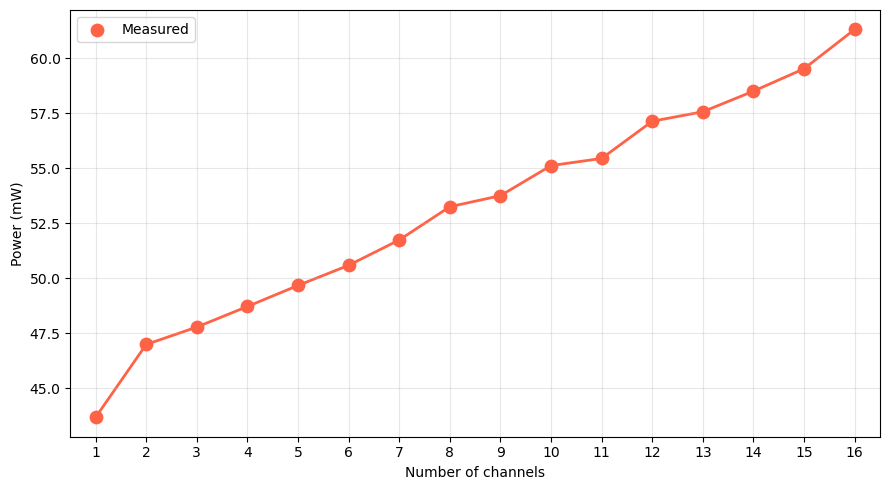
\includegraphics[width=0.85\textwidth]{figures/power_consumption_at_2kHz_per_channel.png}
    \caption{Combined nRF52832 and Intan RHS2116 power consumption at 3.6\,V as a
    function of the number of active recording channels, all configured at
    2\,kHz per channel. Power increases approximately linearly with channel count
    (43.7\,mW for 1 channel to 61.3\,mW for 16 channels). The 1-channel case
    falls below the trend due to the lower SPI transaction rate in single-channel
    mode (2\,kHz) compared to multi-channel mode (32\,kHz total).}
    \label{fig:power_2khz}
\end{figure}

\subsubsection*{Maximum achievable rate and power vs.\ channel count}

Figure~\ref{fig:power_maxrate} shows the maximum achievable per-channel sampling
rate and the corresponding combined power consumption as a function of channel
count. For 4--16 channels the system is BLE-limited: the total useful throughput
is capped at 32\,000 samples/s, and per-channel rate decreases inversely with
channel count. For 2 and 3 channels the system is instead SPI-limited: the SPI
bus reaches its empirical maximum of 128\,kHz, yielding 8\,kHz per channel, but
the resulting BLE throughput (16\,000 and 24\,000 samples/s respectively) is
below the 32\,000\,samples/s BLE ceiling. The reduced BLE activity produces a
visible dip in power for these two configurations.

The 1-channel configuration at its maximum rate of 32\,kHz per channel has the
same SPI rate (32\,kHz) and BLE throughput (32\,000 samples/s) as the
16-channel, 2\,kHz configuration, and would therefore be expected to show
comparable power. The measured value is somewhat higher; a likely contributor
is the difference in Intan RHS2116 register configuration between single-channel
mode (\texttt{CONVERT($k$)}) and multi-channel mode (\texttt{CONVERT(63)}),
though this has not been confirmed. \TODO{Revisit once 3.0\,V vs 3.6\,V data are available; check whether Convert(k) consistently draws more power than Convert(63) across repeated measurements.}

\begin{figure}[h]
    \centering
    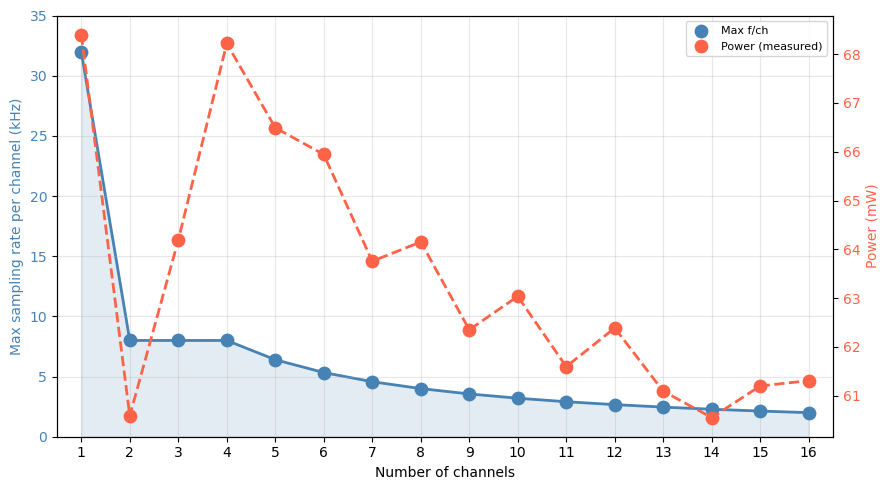
\includegraphics[width=0.85\textwidth]{figures/max_rate_per_channel_and_power_consumption.png}
    \caption{Maximum achievable per-channel sampling rate (left axis, circles) and
    combined nRF52832 and Intan RHS2116 power consumption at 3.6\,V (right axis,
    squares) as a function of the number of active recording channels. Configurations
    with 4--16 channels are BLE-limited at 32\,000 total samples/s; 2 and 3 channels
    are SPI-limited at 128\,kHz and show a dip in power due to lower BLE throughput.}
    \label{fig:power_maxrate}
\end{figure}

\subsubsection*{Power consumption time course}

Figure~\ref{fig:power_timecourse} shows the power consumption over time for the
1-channel, 2\,kHz per channel configuration at 3.6\,V. The full 2.866\,s trace
(top) reveals eight periodic spikes with an inter-spike interval of approximately
400\,ms. This matches the expected DMA buffer-swap period exactly: in
single-channel mode at 2\,kHz, one SPI transaction occurs every 500\,\textmu{}s,
so the Timer2 threshold of 819 transactions fires after $819 \times 500\,\mu\text{s}
= 409.5\,\text{ms}$. Each spike peaks at approximately 27\,mA (97\,mW at 3.6\,V),
reflecting the combined cost of copying the inactive DMA buffer into the ring buffer
and assembling and transmitting the BLE packets.

The 40\,ms zoomed window (bottom) resolves the BLE connection-event structure.
Five peaks appear at 10\,ms intervals, confirming the empirically negotiated
connection interval. Each event shows a double-peak structure: a smaller peak
($\approx$15\,mA, 54\,mW) followed approximately 1.5\,ms later by a larger peak
($\approx$19\,mA, 68\,mW), consistent with the sequential radio interrupts within
a single connection event described in Appendix~\ref{app:softdevice_timing}.

\begin{figure}[h]
    \centering
    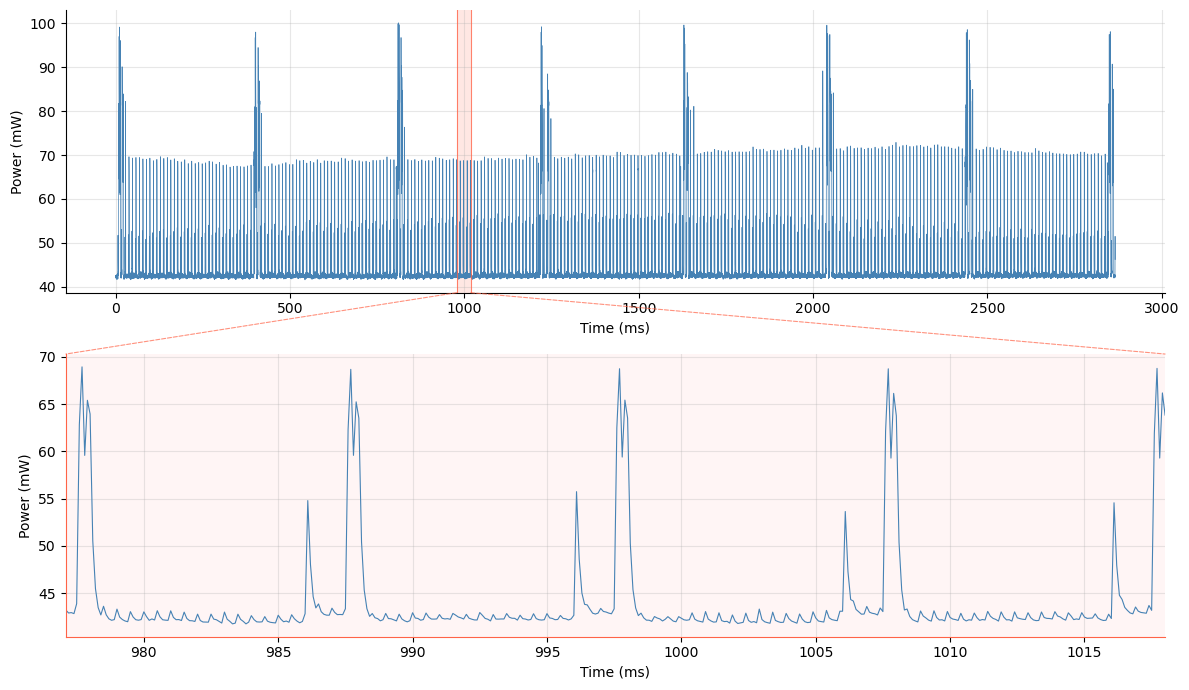
\includegraphics[width=\textwidth]{figures/power_consumption_1ch_2kHz.png}
    \caption{Power consumption time course for the 1-channel, 2\,kHz per channel
    configuration at 3.6\,V (Intan RHS2116\,+\,WLCSP49 nRF52832 module).
    \textit{Top:} full 2.866\,s trace showing eight periodic DMA buffer-swap spikes
    (peak $\approx$97\,mW) with an interval of approximately 400\,ms, consistent
    with the Timer2 threshold period of $819 \times 500\,\mu\text{s} = 409.5\,\text{ms}$.
    The shaded region indicates the zoomed segment.
    \textit{Bottom:} 40\,ms zoom revealing BLE connection events at the negotiated
    10\,ms interval. Each event exhibits a double-peak structure (54\,mW then
    68\,mW) corresponding to sequential SoftDevice radio interrupts within the same
    connection event.}
    \label{fig:power_timecourse}
\end{figure}

The large periodic spikes arise from the CPU work at each DMA buffer swap: copying
819 sample-entries from the inactive DMA buffer into the ring buffer and preparing
BLE packets. An alternative architecture could send data directly from the inactive
DMA buffer without an intermediate ring buffer, potentially eliminating these
spikes. However, this trade-off has two costs. First, the ring buffer stores only the selected channels at 2\,bytes per sample, while
the DMA buffers hold all 16 channels at 4\,bytes each. Even in the 16-channel
case the ring buffer is 2$\times$ more memory-efficient per sample (2 vs.\ 4\,bytes);
in a 2-channel recording --- the worst case --- it is 16$\times$ more efficient
(2\,channels $\times$ 2\,bytes $=$ 4\,bytes per cycle vs.\
16\,channels $\times$ 4\,bytes $=$ 64\,bytes), allowing a proportionally longer
recording to be buffered in the same memory. The overall system holds both the DMA
buffers and the ring buffer simultaneously, so the system-level gain is smaller
than these per-buffer ratios suggest. Second, removing the ring buffer
reintroduces a synchronisation problem between the SPI EasyDMA write path and the
BLE read path, requiring careful atomic coordination that the current architecture
cleanly avoids. This optimisation is therefore left for future work if power
becomes the primary design constraint.

\subsection{Electromagnetic Interference in the WPT Field}
\label{sec:results_noise}

\TODO{}


\begin{comment}
\subsection{SPI Transaction Time Measurement}

Figure~\ref{fig:spi_burst_cursors} shows the oscilloscope cursor measurement 
used to determine the SPI transaction time. Cursors were placed at the start 
and end of a burst of 67 consecutive SPI transactions, yielding a total burst 
duration of 346\,\textmu s and a mean transaction time of 5.164\,\textmu s 
(Equation~\ref{eq:spi_transaction_time}). The built-in Period measurement 
function confirmed a value in the same range but exhibited cycle-to-cycle 
jitter, motivating the use of the cursor-based aggregate measurement as the 
calibration value.

\begin{figure}[htbp]
    \centering
    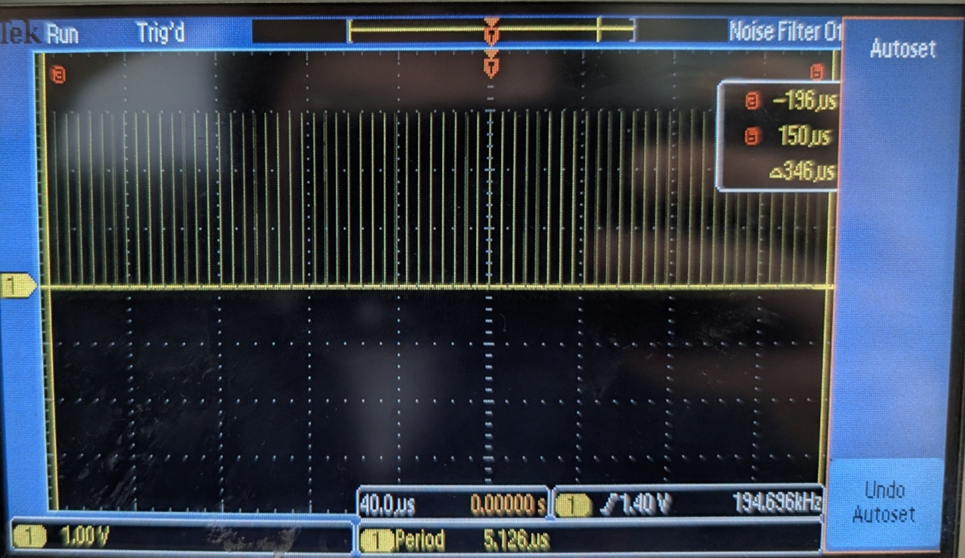
\includegraphics[width=0.6\textwidth]{figures/spi_burst_cursors.png}
    \caption{Oscilloscope cursor measurement of 67 consecutive SPI transactions 
    on the Tektronix DPO~2024. The total burst duration of 346\,\textmu s 
    yields a mean transaction time of $346/67 = 5.164$\,\textmu s, used as 
    the calibration constant \texttt{SPI\_TRANSACTION\_TIME\_US} in the 
    stimulation firmware.}
    \label{fig:results_spi}
\end{figure}

\subsection{Stimulation Waveform Validation}
\label{sec:results_stim}

Figure~\ref{fig:stim_oscilloscope} shows the biphasic stimulation waveform 
measured at the Intan RHS2116 output using the Tektronix DPO~2024 oscilloscope. 
The waveform exhibits the expected charge-balanced biphasic shape: a cathodic 
(negative) phase, followed by an interphase gap, and an anodic (positive) phase. 
The measured phase durations and amplitudes are consistent with the parameters 
configured in the GUI stimulation interface (Figure~\ref{fig:stim_gui}).

\begin{figure}[htbp]
    \centering
    \begin{subfigure}[b]{0.53\textwidth}
        \centering
        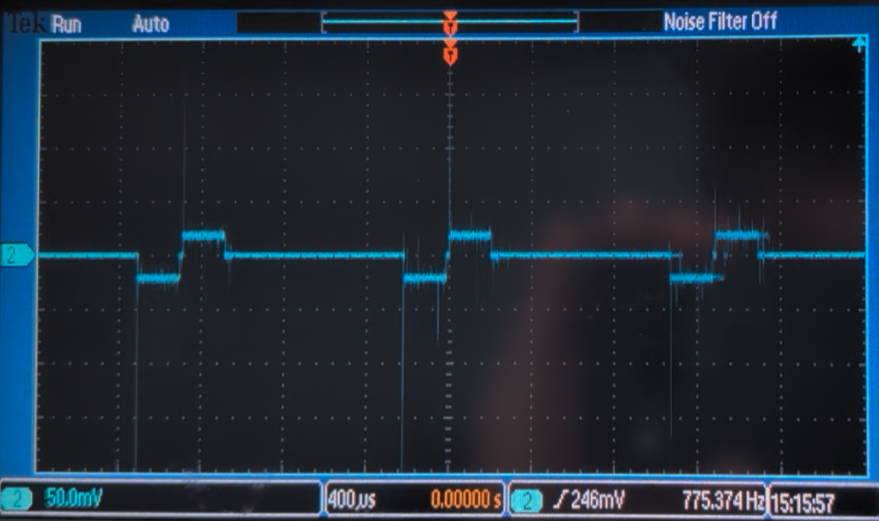
\includegraphics[height=5cm]{figures/oscilloscope_stim.png}
        \caption{Oscilloscope trace of the biphasic stimulation waveform.}
        \label{fig:stim_oscilloscope}
    \end{subfigure}
    \hfill
    \begin{subfigure}[b]{0.43\textwidth}
        \centering
        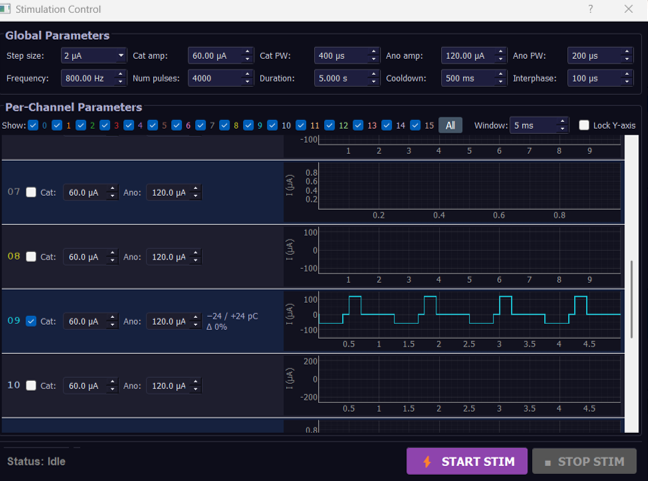
\includegraphics[height=5cm]{figures/gui_stim_window.png}
        \caption{Corresponding stimulation parameters as configured 
        in the GUI.}
        \label{fig:stim_gui}
    \end{subfigure}
    \caption{Stimulation waveform validation. The oscilloscope trace 
    confirms correct biphasic pulse shape, timing, and charge balance 
    consistent with the GUI-configured parameters.}
    \label{fig:stim_combined}
\end{figure}

\subsection{Neural Signal Recording}

Figure~\ref{fig:gui_recording} shows a screenshot of the GUI during live 
16-channel recording from the Intan RHS2116. All 16 channels are displayed 
simultaneously at 2\,kHz per channel, with real-time packet loss monitoring 
visible in the status bar.

\begin{figure}[h]
    \centering
    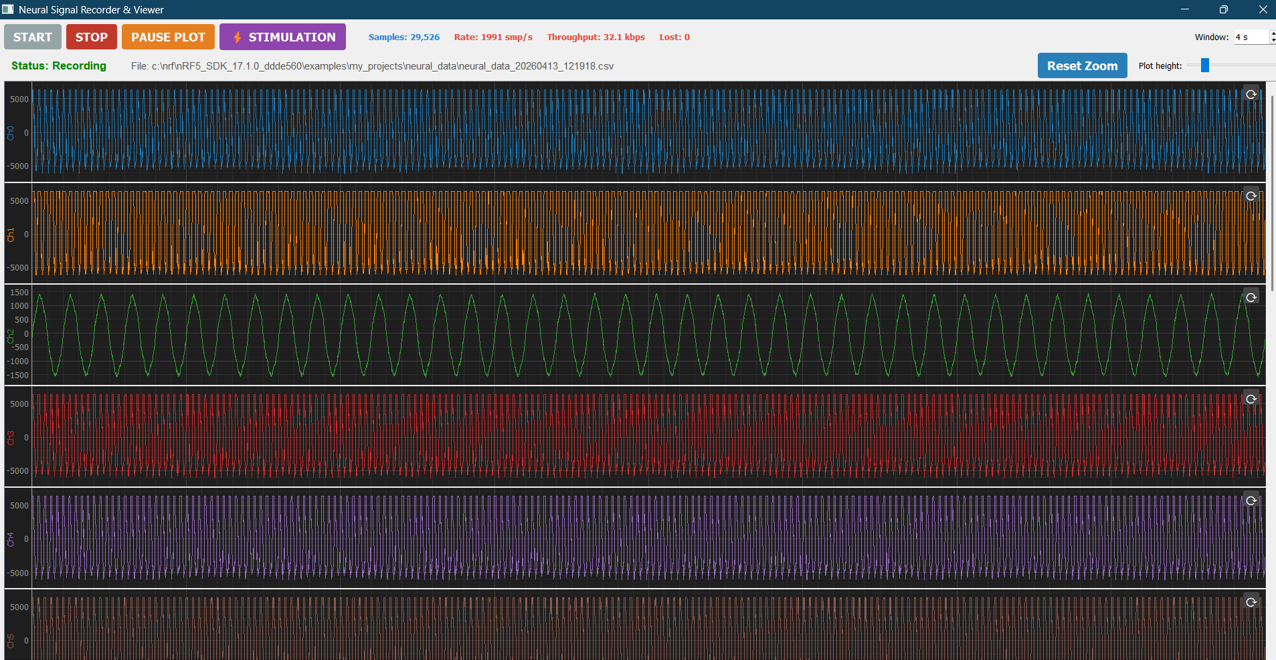
\includegraphics[width=\textwidth]{figures/gui_recording.png}
    \caption{GUI screenshot during live 16-channel neural signal recording. 
    Voltage traces for all 16 Intan RHS2116 channels are rendered in real 
    time at 2\,kHz per channel. The status bar displays throughput and 
    packet loss metrics.}
    \label{fig:gui_recording}
\end{figure}

\end{comment}